\documentclass[11pt]{article}
\usepackage[letterpaper,margin=1in]{geometry}
\usepackage{mathptmx}
\usepackage{color}
\usepackage{colortbl}
\usepackage{array}
\usepackage{longtable}
\usepackage{graphicx}
\usepackage{fancyhdr}
\usepackage{url}
% hyperref unavailable in packaging TeX (pdftexcmds missing); urls via url package

\definecolor{navy}{RGB}{20,60,140}
\definecolor{lightnavy}{RGB}{225,233,248}

\renewcommand{\baselinestretch}{1.10}
\emergencystretch=2.5em
\sloppy
\setlength{\parskip}{4pt plus 1pt}
\setlength{\parindent}{0pt}

\makeatletter
\renewcommand{\section}{\@startsection{section}{1}{\z@}%
  {3.2ex plus 1ex minus .2ex}{2.0ex plus .2ex}{\Large\bfseries\color{navy}}}
\renewcommand{\subsection}{\@startsection{subsection}{2}{\z@}%
  {2.6ex plus 1ex minus .2ex}{1.4ex plus .2ex}{\large\bfseries\color{navy}}}
\renewcommand{\subsubsection}{\@startsection{subsubsection}{3}{\z@}%
  {2.2ex plus 1ex minus .2ex}{1.0ex plus .2ex}{\normalsize\bfseries}}
\makeatother

\pagestyle{fancy}
\fancyhf{}
\renewcommand{\headrulewidth}{0pt}
\fancyfoot[C]{\small\thepage}
\fancyhead[L]{\begin{picture}(0,0)\put(-44,-726){\color{navy}\framebox(549,726){}}\end{picture}}
\fancyhead[R]{\small\itshape DOC-1-034 R1 $\cdot$ locked-gate cellulase discovery}

\newcommand{\gatebox}[1]{\par\vspace{6pt}\noindent\fcolorbox{navy}{lightnavy}{\parbox{0.965\linewidth}{#1}}\vspace{6pt}}

\begin{document}

% ============================ TITLE PAGE ============================
\thispagestyle{empty}
\begin{picture}(0,0)\put(-43,-721){\color{navy}\framebox(545,717){}}\end{picture}
\vspace*{0.8cm}
\begin{center}
{\color{navy}\rule{\linewidth}{2.5pt}}\\[10pt]
{\LARGE\bfseries 1,433 computational cellulase candidates,\\[4pt] catalytic-residue intact, from the global metagenome}\\[12pt]
{\large A CAZyme-aware discovery screen with locked gates\\[2pt] and decoy-controlled specificity}\\[10pt]
{\color{navy}\rule{\linewidth}{2.5pt}}
\end{center}
\vspace{1.1cm}
\begin{center}
\begin{tabular}{c}
\large Science Program DOC-1-034 (SP-004), Round 1\\[6pt]
\large Packaging backfill: publication-length synthesis\\[6pt]
\large Protocol locked 2026-09-21 21:24 IST, before any\\ candidate-level result was inspected\\[6pt]
\large Locked-gate outcome: \textbf{OVERALL PASS, 6 of 6 gates}\\
\end{tabular}
\end{center}
\vspace{1.0cm}
\gatebox{\small\textbf{Claims boundary (locked, verbatim from the protocol).} Computational nomination only. No enzymatic activity is claimed for any candidate; no wet-lab validation was performed. Candidates are ranked hypotheses for experimental follow-up in biofuel enzyme-cocktail development.}
\vfill
\begin{center}
{\small Package DOC-1-034-R1 $\cdot$ compiled from frozen R1 artifacts only\\
scientific bytes and claims frozen $\cdot$ audit CLI and manifests included}
\end{center}
\clearpage

% ============================ ABSTRACT ============================
\section*{Abstract}
\addcontentsline{toc}{section}{Abstract}
Cellulosic-biofuel economics are enzyme-cost-limited, and the discovery of diverse cellulases---especially the exo-acting cellobiohydrolases that limit crystalline-cellulose saccharification---remains a bottleneck. We screened the MGnify30-C2 catalog (128.7M non-singleton proteins) with a 15-member, live-verified, CAZyme-family-spanning reference panel under a success gate locked before any candidate-level result was inspected: length, cellulase-GH Pfam-domain, homology ($E \le 10^{-10}$), novelty ($<$40\% identity to every reference), and catalytic Asp/Glu conservation at UniProt-annotated active-site positions, with three non-cellulase decoy panels (xylanase, lysozyme, amylase) run through the identical funnel as a specificity control. The screen yields 1,433 distinct computational cellulase candidates passing the locked F1/F2/F3/F4/F6 filters, all conserving the annotated catalytic Asp/Glu residues; 1,389 of them (96.9\%) sit below 30\% identity to every one of the 15 references, where novelty is defined operationally against that locked panel alone. Decoy yield is zero. No biochemical activity has been established for any candidate. Cross-catalog replication in the independent Pfam-poor MGnify30-C5-ppfam catalog recovers 30 candidates under the identical funnel, and composition-preserving scrambled controls produce zero hits against the full catalog. Structure templates at $E \le 10^{-10}$ with $\ge$60\% coverage exist for 16 of the top-50 candidates. The pool is compositionally asymmetric in a commercially meaningful way: 84\% are endoglucanases (GH5) and beta-glucosidases (GH3), while exo-acting cellobiohydrolases are scarce (GH7 3.0\%, GH6 7.6\%, GH48 1.3\%)---identifying the 171-candidate exo-acting tranche as the high-value feedstock for cocktail engineering and the 672 beta-glucosidases as a screening library for glucose-tolerant variants. All gates, thresholds, decoy rules, and the failure policy were locked before results were seen; all six locked gates pass.

\medskip
\noindent\textbf{Keywords:} cellulase; cellobiohydrolase; metagenome mining; MGnify; glycoside hydrolase; locked-gate validation; decoy controls; cellulosic biofuel; enzyme cocktail; computational discovery

% ============================ 1 INTRO ============================
\section{Introduction}

\subsection{The enzyme-cost bottleneck in cellulosic biofuels}
Enzymatic saccharification converts pretreated lignocellulose to fermentable sugars using cocktails of endoglucanases (EG; families GH5, GH7, GH12, GH45), exo-cellobiohydrolases (CBH; GH7 CBH1 and GH6 CBH2), beta-glucosidases (BGL; GH1, GH3), and processive accessory enzymes (GH9, GH48) [1, 2, 38--42]. Industrial cocktails derive overwhelmingly from a small number of fungal hosts---\textit{Trichoderma reesei} above all---and the cost of the enzyme cocktail per gallon of cellulosic ethanol remains a primary economic lever for the industry [3, 4]. Two activities dominate the cost structure: the exo-acting cellobiohydrolases that attack crystalline cellulose and account for the largest protein share of commercial cocktails [5, 6], and the beta-glucosidases that relieve cellobiose inhibition and complete hydrolysis to glucose [7].

\subsection{Metagenomes as a discovery reservoir}
Metagenomic sequence catalogs sample microbial dark matter at a scale that dwarfs the characterized-enzyme literature. The MGnify resource aggregates tens of millions of non-redundant proteins from environmental sequencing [8, 9, 50], and global marine surveys keep expanding the bioprospecting reservoir [28], and metagenomic cellulase discovery has repeatedly delivered industrial candidates, including thermostable enzymes from hot environments, oil reservoirs, soda lakes, and extreme terrestrial sites [10--15]. The limiting step is no longer finding homologs; it is deciding which homologs are worth expressing.

\subsection{Specificity is the discovery problem}
The discovery problem is therefore not sensitivity---cellulases are abundant in environmental sequence---but specificity and validation. Glycoside hydrolases share folds and catalytic machinery across substrate classes: xylanases, amylases, and lysozymes are mechanistically adjacent to cellulases [16, 17], so a sequence-similarity screen that is not family-aware risks family-bleed false positives. Candidate lists assembled without decoy controls, catalytic-residue verification, and independent replication are not decision-grade, and sequence identity alone is a weak basis for function transfer in the twilight zone [18, 19].

\subsection{This study}
We therefore designed and locked a CAZyme-family-aware discovery protocol before inspecting any candidate: a reference panel of 15 characterized cellulases spanning 8 GH families with UniProt \texttt{ACT\_SITE} grounding; catalytic acid/base conservation as an explicit filter; three non-cellulase decoy panels processed through the identical funnel; independent-catalog replication; composition-preserving scrambled-sequence controls; and a predeclared six-gate success criterion with a written failure policy. The screen returns 1,433 computational cellulase candidates passing every locked filter from 128.7M metagenomic proteins, and the locked decoy design is what makes that count meaningful. Section 2 states the hypothesis and the locked gates; Section 3 describes methods; Section 4 reports results; Section 5 discusses the commercial and discovery implications; Sections 6--8 cover limitations, reproducibility, and availability.

% ============================ 2 HYPOTHESIS AND GATES ============================
\section{Hypothesis and locked success gates}

\subsection{Locked question}
The protocol (locked 2026-09-21 21:24 IST; SHA-256 \texttt{a90624ce\ldots c17d}, reproduced in Appendix~A) asks: does the MGnify metagenomic protein catalog contain glycoside-hydrolase cellulase homologs that (a) retain the catalytic machinery of characterized cellulase GH families, (b) carry cellulase-family Pfam domains, (c) are substantially sequence-divergent from every experimentally characterized cellulase in the reference panel, and (d) retain structural template support in the PDB?

\subsection{The six gates}
Gate text was frozen before any hit table was inspected and was never modified afterward. The frozen gate record is \texttt{results/gate\_evaluation.json}; the packaged audit CLI re-derives every observed count from the frozen candidate tables and compares it against this record field-for-field (Section~7).

\begin{table}[h]
\centering\small
\arrayrulecolor{navy}
\begin{tabular}{|p{0.5cm}|p{7.6cm}|p{2.0cm}|p{2.6cm}|p{1.3cm}|}
\hline
\rowcolor{lightnavy}\textbf{Gate} & \textbf{Locked rule (abbrev.)} & \textbf{Threshold} & \textbf{Observed} & \textbf{Verdict} \\\hline
G1 & live-verified characterized cellulase references & $\ge$12 & 15 & PASS \\\hline
G2 & distinct MGnify candidates pass F1, F2, F3, F4, F6 & $\ge$40 & 1,433 & PASS \\\hline
G3 & of G2, novelty $<$30\% to every reference & $\ge$15 & 1,389 & PASS \\\hline
G4 & of top-50 examined, RCSB template $E\le10^{-10}$ and coverage $\ge$60\% & $\ge$15 & 16/50 & PASS \\\hline
G5 & thermostability proxy (aliphatic index $\ge$ reference median 64.44 and $\ge$2 Cys) & $\ge$5 & 1,266 & PASS \\\hline
G6 & decoy pools yield $\le$10\% of reference yield & $\le$9.55/query & 0/query (ref.\ 95.5/query) & PASS \\\hline
\end{tabular}
\caption{Locked success gates and outcomes (frozen record: \texttt{results/gate\_evaluation.json}).}
\end{table}

Positive controls were locked alongside the gates: C1 requires $\ge$85\% of the 15 references to pass the length window F1 (validating the window), and C3 is the decoy-specificity control formalized as gate G6. The locked failure policy states that if any required gate fails, the project is classified as negative, all raw artifacts, hit tables, rejected sets, and figures are preserved, and no success paper is produced. Leakage controls locked at the same time include: gates and thresholds locked before any hit table is inspected; the reference panel fixed before searching; the Pfam catalytic set fixed from the panel's own live annotations; raw API responses hashed (SHA-256) at download with results derived only from hashed artifacts; and decoy pools processed identically but counted separately, with no simulated data.

% ============================ 3 METHODS ============================
\section{Methods}

\subsection{Reference panel (grounding-first)}
Fifteen experimentally characterized cellulases spanning CAZy families GH3, GH5, GH6, GH7, GH9, GH12, GH45, and GH48 were retrieved live from UniProtKB and RCSB on 2026-09-21, each verified to carry active-site (\texttt{ACT\_SITE}) feature annotations, Pfam cross-references, and (mostly) PDB structures; mature sequences were used with signal peptides removed where annotated (Appendix~B). Panel construction was grounding-first rather than recall-first: the initial name-based queries (for example, protein name ``Cellobiohydrolase 1'' in \textit{T.\ reesei}) returned zero hits under the exact names first tried, so the panel was rebuilt from live organism-level queries instead of recalled accessions, and the raw query JSON and FASTA responses were hashed at fetch time (feasibility log, \texttt{protocol/feasibility\_log.md}). One panel member, the \textit{Pyrococcus furiosus} endoglucanase (Q9V2T0), carries no \texttt{ACT\_SITE} annotation; this was recorded before locking, and the catalytic filter routes around it via the next-best annotated reference. CAZy mechanism pages (retaining vs.\ inverting per GH family) were downloaded and hashed into the grounding set. Three decoy hydrolases from non-cellulase glycosidase families were verified live in the same session: \textit{T.\ reesei} xylanase~1 (P36218, GH11), hen lysozyme~C (P00698, GH22), and \textit{Bacillus licheniformis} alpha-amylase (P06278, GH13).

\subsection{Search}
Each of the 15 mature reference sequences and the 3 decoys was searched against the MGnify30-C2 non-singleton catalog using phmmer via the EBI HMMER API v1 [20, 21, 51]. All hits with $E \le 10^{-5}$ to at least one reference were collected, unioned across references, and deduplicated by MGYP accession, yielding 12,451 unique reference hits; decoy hits were kept in a separate pool (1,273 hits). The database version was recorded at run time (\texttt{2026\_07}; $Z = 128{,}674{,}267$ sequences), and every HMMER job UUID, status, and statistics block is preserved in \texttt{results/run\_manifest\_ref.json} and \texttt{results/run\_manifest\_decoy.json}.

\subsection{Locked filters}
\begin{table}[h]
\centering\small
\arrayrulecolor{navy}
\begin{tabular}{|p{0.9cm}|p{13.6cm}|}
\hline
\rowcolor{lightnavy}\textbf{Filter} & \textbf{Locked rule} \\\hline
F1 & length 180--900 amino acids (covers the reference-panel span 213--880 aa, including multi-domain cellulases) \\\hline
F2 & candidate Pfam annotations (MGnify hit metadata) must include at least one catalytic cellulase-GH family from the locked set \{PF00150 GH5, PF01341 GH6, PF00840 GH7, PF00759 GH9, PF01670 GH12, PF02015 GH45, PF02011 GH48, PF01915 GH3\}; candidates with no Pfam annotation are recorded as not-evaluable and excluded from gate counts \\\hline
F3 & minimum phmmer E-value across the 15 references $\le 10^{-10}$ \\\hline
F4 & maximum global pairwise identity to any of the 15 references $<$40\%; Biopython PairwiseAligner global, BLOSUM62, open $-11$, extend $-1$; identity = identical positions / alignment columns \\\hline
F6 & every annotated catalytic position of the candidate's best-E \texttt{ACT\_SITE} reference must align to Asp or Glu in the candidate; candidates whose reference hits all lack \texttt{ACT\_SITE} annotation are recorded not-evaluable and excluded from gate counts \\\hline
F5 & top 50 F1--F4+F6 survivors by E-value: RCSB sequence search $E \le 10^{-10}$ plus local-alignment coverage $\ge$60\% of candidate length \\\hline
\end{tabular}
\caption{Locked filter definitions (verbatim from \texttt{protocol/protocol.json}).}
\end{table}

\subsection{Documented execution substitution: the F6 mapping vehicle}
The locked F6 rule names the phmmer aligned-FASTA (afa) as the position-mapping vehicle. During execution it was verified on the downloaded files that EBI afa downloads contain only hit rows---the query/reference row is absent (543/543 headers are MGYP hits)---so a reference-position-to-column mapping cannot be built from the afa. The locked rule itself (D/E at every annotated catalytic position of the best-E \texttt{ACT\_SITE} reference) is unchanged; the mapping is computed from a pairwise global alignment against that same reference using the identical BLOSUM62 $-11/{-1}$ aligner as F4. The substitution was recorded at run time in the report and in code; the gate text was not touched. Its conservative consequence is analyzed in Sections 5 and 6.

\subsection{Stage-2 validation}
Three independent validation arms were predeclared and run after the primary funnel: (A)~\textbf{cross-catalog replication}---the full 15-reference screen rerun against the independent MGnify30-C5-ppfam catalog with the identical F1--F4 funnel; C5-ppfam specifically holds sequences poor in Pfam annotations, so F2 is harder to satisfy there by construction and the arm is a deliberately hard replication set. (B)~\textbf{scrambled controls}---composition-preserving shuffles of 5 final candidates searched against the full MGnify30-C2 catalog. (C)~\textbf{UniProt novelty screen}---the top-20 final candidates searched by phmmer against UniProtKB with best-homolog identity recorded, testing novelty beyond the 15-member reference panel. No gate depends on arm C.

\subsection{Structure modelability and thermostability proxy}
The top-50 final candidates by E-value were queried against RCSB by sequence search; a qualifying template requires $E \le 10^{-10}$ and local-alignment coverage $\ge$60\% of candidate length (gate G4); the cellobiohydrolase and endoglucanase template space is structurally well charted [33--37, 43--46]. The thermostability proxy (gate G5) is a sequence-derived screen, not a measurement: aliphatic index $\ge$ the reference-panel median (64.44) and $\ge$2 cysteine residues.

\subsection{Provenance and locking mechanics}
All retrievals---UniProt entries and feature tables, RCSB FASTAs, CAZy family pages, EBI HMMER jobs, PubMed eutils---were hashed (SHA-256) at fetch time, and results derive only from hashed artifacts. The locked protocol hash is embedded in the frozen gate record (\texttt{results/gate\_evaluation.json}), and the packaged protocol file reproduces that hash exactly:
\begin{center}\small\texttt{a90624ce91b33a59519677523df712047c86e977cc863ae9a164bb117079c17d}\end{center} Literature grounding was retrieved live from NCBI eutils on 2026-09-21; the full query-and-hit ledger is \texttt{report/literature\_ledger.md}, and the reference list of this paper is drawn from it.

% ============================ 4 RESULTS ============================
\section{Results}

\subsection{A specificity-controlled funnel: 12,451 hits to 1,433 candidates}
The 15-reference phmmer screen against MGnify30-C2 returned 12,451 unique hits at $E \le 10^{-5}$. The locked filters reduce these to 1,433 final candidates (Figure~1, Table~3): 9,057 pass the length window (F1); 5,033 carry a locked cellulase-GH Pfam domain (F2, with 269 hits not evaluable for lack of Pfam metadata and excluded from gate counts by design); 3,401 pass the homology threshold $E \le 10^{-10}$ (F3); 3,395 pass the novelty filter $<$40\% identity to every reference (F4); and 1,433 conserve Asp/Glu at every annotated catalytic position of their best-E \texttt{ACT\_SITE} reference (F6). The three decoy pools returned 1,273 raw hits, of which 848 pass F1 and \textbf{zero} carry a cellulase-GH Pfam domain---so the identical funnel produces zero gate-counted decoy candidates (gate G6).

\begin{figure}[h]
\centering
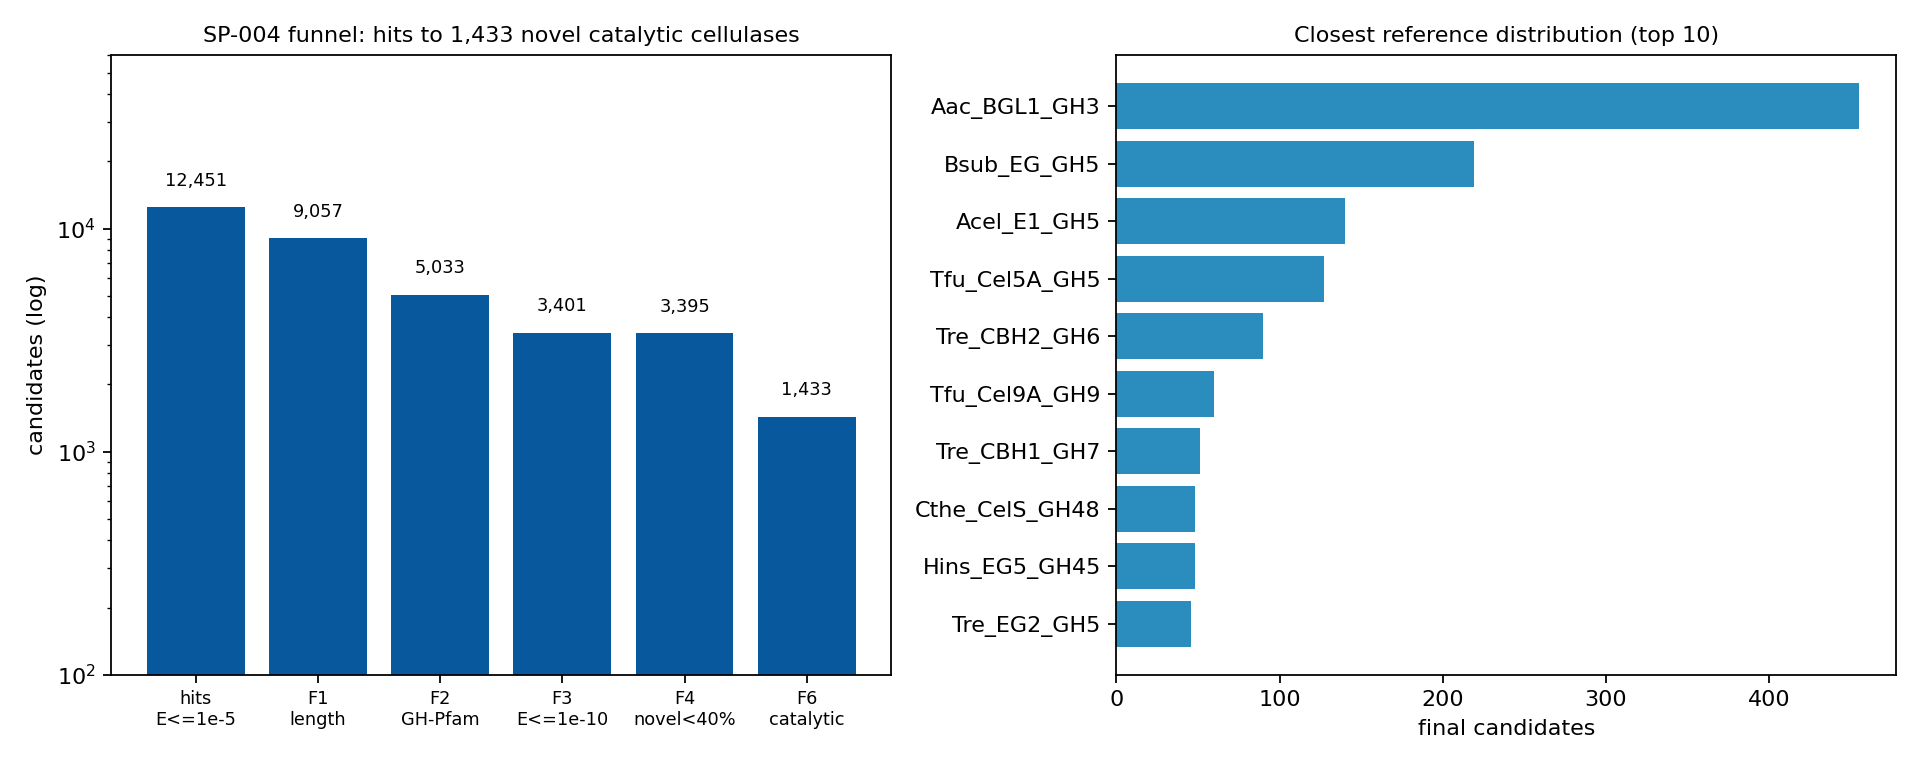
\includegraphics[width=\linewidth]{../figures/sp004_funnel.png}
\caption{Left: the locked discovery funnel from 12,451 unique hits ($E \le 10^{-5}$) to 1,433 final candidates (log scale). Right: closest-reference distribution of the final candidates (top 10 of 15 references); no single reference dominates the pool. (Frozen figure: \texttt{figures/sp004\_funnel.png}.)}
\end{figure}

\begin{table}[h]
\centering\small
\arrayrulecolor{navy}
\begin{tabular}{|l|r|r|}
\hline
\rowcolor{lightnavy}\textbf{Stage} & \textbf{Reference pool} & \textbf{Decoy pool} \\\hline
unique hits ($E \le 10^{-5}$, deduplicated) & 12,451 & 1,273 \\\hline
F1 length 180--900 aa & 9,057 & 848 \\\hline
F2 cellulase-GH Pfam & 5,033 & 0 \\\hline
F3 $E \le 10^{-10}$ & 3,401 & 0 \\\hline
F4 $<$40\% identity to every reference & 3,395 & 0 \\\hline
F6 catalytic D/E intact & \textbf{1,433} & \textbf{0} \\\hline
\end{tabular}
\caption{Funnel counts for the reference and decoy pools (frozen: \texttt{results/funnel\_ref.json}, \texttt{results/funnel\_decoy.json}). The decoy funnel terminates at F2: no decoy hit carries a cellulase-GH Pfam domain.}
\end{table}

\subsection{All six locked gates pass}
Gate G1 is satisfied by the 15-member live-verified panel (threshold 12). G2 is satisfied by 1,433 distinct candidates (threshold 40). G3 is satisfied by 1,389 candidates below 30\% identity to every reference (threshold 15). G4 is satisfied by 16 of the top-50 candidates with qualifying RCSB templates (threshold 15). G5 is satisfied by 1,266 candidates passing the thermostability proxy (threshold 5). G6 is satisfied with a decoy yield of 0 per query against a reference yield of 95.5 per query (threshold $\le$9.55). The frozen gate record reports \texttt{overall: PASS}; the audit CLI reproduces every observed number in it from the packaged tables (Section~7).

\subsection{The candidates are divergent from characterized references and catalytic-residue intact}
Of the 1,433 final candidates, 1,389 (96.9\%) sit below 30\% global identity to every characterized reference, and the full set is below 40\% (Figure~2). Every candidate conserves Asp or Glu at every annotated catalytic position of its best \texttt{ACT\_SITE} reference---the catalytic acid/base machinery is intact by construction of F6. The predeclared novelty sensitivity tabulation (Appendix~D) shows the count is robust across the locked threshold neighborhood: 1,253 candidates remain below even a 25\% identity cutoff.

\begin{figure}[h]
\centering
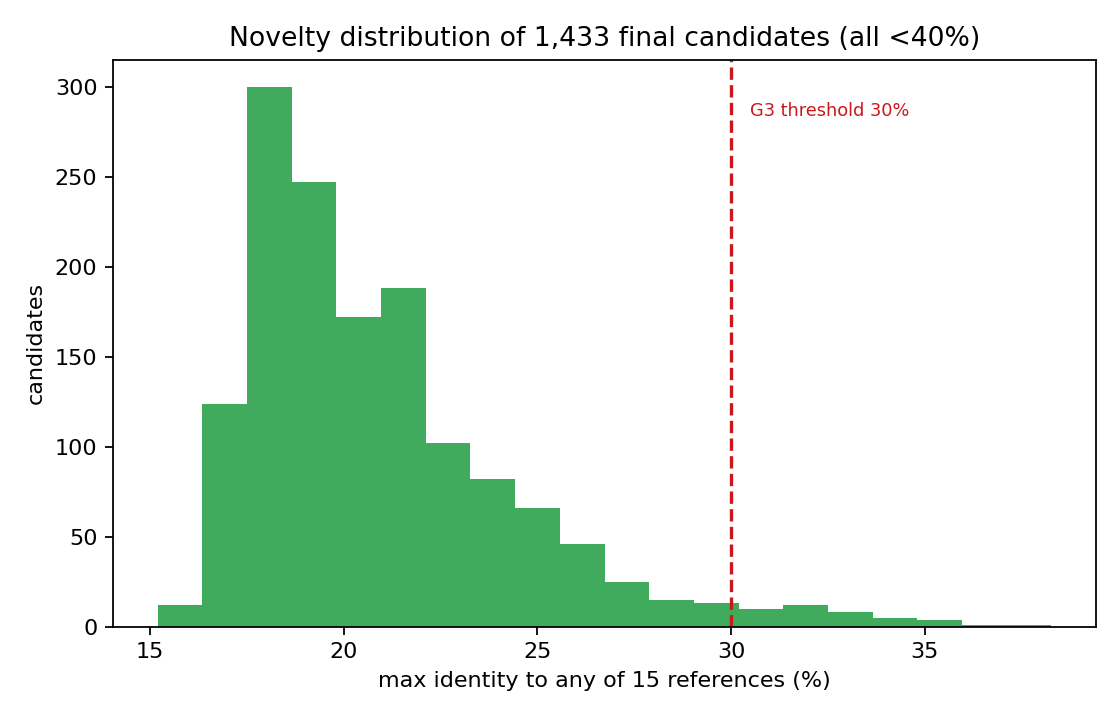
\includegraphics[width=0.86\linewidth]{../figures/sp004_novelty.png}
\caption{Novelty distribution of the 1,433 final candidates: maximum global identity to any of the 15 references (all $<$40\% by F4). The dashed line marks the locked G3 threshold at 30\%; 1,389 candidates (96.9\%) fall below it. (Frozen figure: \texttt{figures/sp004\_novelty.png}.)}
\end{figure}

UniProtKB screening of the top-20 candidates (stage-2 arm C) probes novelty beyond the 15-member panel, with mixed results: across the 15 completed screens the median best-homolog identity is 36.1\% (range 2.2--100\%). Three candidates match existing metagenome-derived UniProt deposits at near-identity (MGYP001480172483 at 99.7\% to A0A370GNA7; MGYP003860412909 at 98.5\% to A0A2T5PCH5; MGYP000843571747 at 100\% to A0A7X7NE49) and are flagged as already-known: they remain in the set but are deprioritized for novelty claims, and they are preserved as novelty negatives for future rounds. One candidate (MGYP007332108226) has no UniProtKB hit at $E \le 10^{-40}$. Five of the 20 screens could not complete because of an EBI HMMER API incident on 2026-09-21/22 (job records purged immediately after submission, verified across three or more resubmissions each) and are documented as such in \texttt{results/uniprot\_screen\_summary.json}; no gate depends on this screen.

\subsection{Compositional asymmetry: the commercial core finding}
The GH-family composition of the pool is strongly asymmetric (Table~4). Beta-glucosidases (GH3, 672 candidates, 46.9\%) and endoglucanases (GH5, 530, 37.0\%) dominate, while the exo-acting cellobiohydrolase classes are scarce: GH6 109 (7.6\%), GH7 43 (3.0\%), GH48 19 (1.3\%). The exo-acting tranche (GH7+GH6+GH48) totals 171 candidates, 11.9\% of the pool. Median candidate length is 604 aa.

\begin{table}[h]
\centering\small
\arrayrulecolor{navy}
\begin{tabular}{|l|l|r|r|}
\hline
\rowcolor{lightnavy}\textbf{GH family} & \textbf{Role in cocktails} & \textbf{Count} & \textbf{Share} \\\hline
GH3 & beta-glucosidase (cellobiose $\to$ glucose) & 672 & 46.9\% \\\hline
GH5 & endoglucanase & 530 & 37.0\% \\\hline
GH6 & cellobiohydrolase II (exo, reducing end) & 109 & 7.6\% \\\hline
GH45 & endoglucanase & 56 & 3.9\% \\\hline
GH7 & cellobiohydrolase I (exo, processive) & 43 & 3.0\% \\\hline
GH48 & processive cellulase (cellulosomal) & 19 & 1.3\% \\\hline
multi-domain & carries $>$1 locked cellulase-GH Pfam & 4 & 0.3\% \\\hline
\end{tabular}
\caption{GH-family composition of the 1,433 final candidates (tabulation of the frozen candidate table). Exo-acting tranche GH7+GH6+GH48: 171 candidates (11.9\%).}
\end{table}

\subsection{Structure modelability and thermostability proxy}
Sixteen of the top-50 candidates have RCSB templates at $E \le 10^{-10}$ with $\ge$60\% local coverage (gate G4; qualifying templates include 6GJF, 5IHS, 4XNN, 8FC0, 1L1Y, 4EL8; the full table is Appendix~C). A further three examined candidates carry 1ECE templates at sub-threshold coverage (57.7\%, 45.3\%, 42.3\%) and are not gate-counted. Qualifying template identities run 43.8--78.6\%, so these 16 meet the locked template-availability criterion and are the natural first tranche for structure-guided triage; no models have been built and no model quality has been assessed. The thermostability proxy (aliphatic index $\ge$ 64.44 and $\ge$2 cysteines) is met by 1,266 of 1,433 candidates (88.3\%); this is a sequence proxy only, and Section~6 lists it as a limitation.

\subsection{Stage-2 validation: replication and negative controls}
\textbf{Cross-catalog replication.} The identical funnel rerun in the independent MGnify30-C5-ppfam catalog recovers 30 candidates, all at $E \le 10^{-10}$ and $<$40\% reference identity (\texttt{results/xcat\_candidates.json}). Because C5-ppfam is Pfam-poor by construction, F2 is harder to satisfy there, so 30 is a lower bound on true replication rather than an estimate of it. \textbf{Scrambled controls.} All 5 composition-preserving scrambled candidates produce zero hits at $E \le 10^{-10}$ against the full 128.7M-sequence catalog (\texttt{results/scramble\_controls.json}), consistent with the funnel's counts not being an artifact of composition or length bias in the search setup; five controls cannot exclude every such artifact, but they remove the trivial version of that explanation. \textbf{Decoys.} As reported above, the three non-cellulase hydrolase pools---mechanistically adjacent enzymes sharing glycoside-hydrolase catalytic chemistry---yield zero gate-counted candidates through the identical funnel.

% ============================ 5 DISCUSSION ============================
\section{Discussion}

\subsection{Why the locked decoy design is what makes the count meaningful}
A phmmer screen of 15 cellulase references against 128.7M proteins will always return thousands of hits; the scientific content of this study is the evidence that the 1,433 surviving candidates carry cellulase-family signatures rather than family bleed. Three control arms bear the weight. First, the decoy panels: xylanase (GH11), lysozyme (GH22), and amylase (GH13) queries---all glycoside hydrolases with shared catalytic chemistry and, for xylanase, an adjacent hemicellulose substrate---produce 1,273 raw hits but zero candidates through the identical funnel, because no decoy hit carries a locked cellulase-GH Pfam domain (F2) [16, 17]. Second, the scrambled controls weigh against the trivial explanation that any cellulose-adjacent composition matches something at this catalog size. Third, cross-catalog replication recovers 30 candidates in an independent, deliberately harder catalog. The claim the data support is precise: a conservative, catalytic-residue-intact, provenance-resolved candidate pool, not biochemical proof of activity for any member.

\subsection{F6 is the discriminating filter, and it is conservative by design}
The catalytic-conservation filter removes 58\% of otherwise-passing homologs (3,395 $\to$ 1,433). The rejected 1,962 sequences are plausibly pseudogene fragments and catalytically degenerate homologs---sequences that look like cellulases to a search engine but show no evidence of conserved catalytic machinery; whether any of them can hydrolyze substrate was not tested. Requiring Asp/Glu conservation at every annotated catalytic position of the best \texttt{ACT\_SITE} reference is a strong functional-intactness screen, and it is deliberately conservative: the documented mapping-vehicle substitution (Section~3.4) can misregister insertions on very distant homologs, which would falsely reject real enzymes rather than falsely accept dead ones. Direct kinetic and mutational maps of the CBH classes [32, 36] say the conserved positions are the load-bearing ones. Combined with the 96.9\% sub-30\%-identity novelty profile, the pool occupies the discovery sweet spot: divergent enough to be uncharacterized, constrained enough to be catalytically credible candidates.

\subsection{The compositional asymmetry is the actionable result}
Metagenomes are rich in endoglucanases and beta-glucosidases and poor in exo-cellobiohydrolases---the same scarcity that makes CBH1 the cost driver of commercial cocktails [5, 6, 22]. Two commercial consequences follow. First, the 171-candidate exo-acting tranche---43 GH7s among them, all catalytic-residue intact and $<$40\% identical to \textit{T.\ reesei} CBH1-class enzymes, 16 of the top-50 candidates meeting the locked structural-template criterion---is direct discovery feedstock for cocktail engineering, where thermostability, product-inhibition tolerance, and lignin tolerance are the engineering targets [4, 8, 23, 49], with cross-species domain exchange an established engineering route [52]. Second, the 672 GH3 beta-glucosidases address the cellobiose-inhibition bottleneck: glucose-tolerant beta-glucosidases are actively sought for cocktail supplementation [7, 24], and 88\% of the pool passes the thermostability proxy, making the GH3 set a screening library rather than a shortlist. The route to use-level is unchanged from the locked plan: shortlist the exo-acting tranche plus thermostable GH3s, express in a fungal or yeast host [25], run microplate saccharification assays on pretreated biomass (filter-paper activity and cellobiose release), and reconstitute cocktails against a commercial baseline under matched protein loading.

\subsection{Relation to prior metagenome cellulase discovery}
Metagenomic cellulase hunts have repeatedly delivered characterized enzymes [10--15], and recent large-catalog studies confirm that environmental sequence space remains undersampled for industrial hydrolases [13, 26, 27]. Mechanistic and machine-learning work on GH7 kinetics, processivity, and sequence-function mapping [29--32] supplies the priors for the structure-guided triage this pool now enables. What distinguishes this resource is not the catalog size but the validation posture: catalytic-residue verification against live \texttt{ACT\_SITE} annotations, decoy-quantified specificity with a locked zero-tolerant threshold, scrambled negative controls, independent-catalog replication, and a novelty screen against all of UniProtKB rather than against the query panel alone---with the three near-identical UniProt deposits disclosed rather than hidden. The pool's weakness is symmetrical with its strength: everything claimed here is computational, and Section~6 is explicit about what remains unmeasured.

\subsection{Reviewer questions and the next computational round}
The project record carries four reviewer questions forward: (1)~do the 171 exo-acting candidates retain activity on crystalline cellulose after expression; (2)~does the family scarcity persist after structure-based adjudication and domain-architecture controls; (3)~can a predeclared structure/register round reduce pairwise catalytic-position misregistration inherited from the F6 substitution; (4)~which candidates improve a commercial baseline cocktail under matched protein loading. Before any wet-lab claim, the planned next round is an orthogonal structure/domain/register pass over the exo-acting tranche with family-stratified controls, independent structure resources, topology and tunnel checks, and frozen pass/failure gates, preserving the three near-identical UniProt deposits as novelty negatives.

% ============================ 6 LIMITATIONS ============================
\section{Limitations}
\begin{itemize}
\item \textbf{Computational nomination only.} No enzymatic activity is claimed for any candidate; no wet-lab validation was performed. Thermostability, cellulose hydrolysis, substrate specificity, expression yield, and cocktail synergy are unmeasured.
\item \textbf{F6 mapping substitution.} The locked afa vehicle was unavailable in EBI downloads (hit rows only), so catalytic positions were mapped through a pairwise global alignment with the identical aligner (Section~3.4). The D/E rule is unchanged, but pairwise mapping on very distant homologs can misregister insertions; the 1,433 are therefore conservative, and the planned structure/register round addresses the residual risk.
\item \textbf{F2 metadata dependence.} F2 depends on MGnify hit-metadata Pfam annotation; 269 hits were not evaluable for F2 and were excluded from gate counts by design, so the funnel may discard real cellulases that lack metadata.
\item \textbf{Structure coverage.} The structure check covers the top-50 only; modelability of the remaining 1,383 candidates is untested.
\item \textbf{Proxy, not measurement.} Gate G5's thermostability criterion is a sequence proxy (aliphatic index and cysteine count), not a biophysical measurement.
\item \textbf{Replication is a lower bound.} The 30 cross-catalog candidates are bounded by C5-ppfam's size and Pfam-poor composition, which also makes F2 harder to satisfy there.
\item \textbf{UniProt screen incompleteness.} 5 of 20 top-candidate UniProtKB screens were blocked by the documented EBI API incident; novelty beyond the panel is established on the 15 completed screens, and 3 of those were already-known deposits.
\item \textbf{Catalog vintage.} Results are bound to MGnify30-C2 version \texttt{2026\_07} and the UniProtKB/RCSB state of 2026-09-21/22; later releases may change novelty and template counts.
\end{itemize}

% ============================ 7 REPRODUCIBILITY ============================
\section{Reproducibility, packaging, and audit}

\subsection{What this package is}
This paper is a packaging-only synthesis of the frozen R1 artifacts: the locked protocol, reports, result tables, figures, and audit records. Scientific bytes and claims are frozen; nothing was reprocessed, rescored, re-thresholded, re-filtered, or augmented with new statistics or new literature-derived claims. Every number in this paper either appears verbatim in a frozen artifact or is a direct tabulation of a frozen table, and the appendices mark which is which.

\subsection{The audit CLI is determination (a): read-only query/audit over frozen outputs}
The packaged tool \texttt{cli/sp004\_audit.py} (Python 3.8+ standard library only, no network) is a \textbf{read-only query/audit interface}, not a rerunnable pipeline wrapper. The determination is (a) rather than (b) for three recorded reasons. First, the original analysis code (\texttt{code/}: \texttt{run\_analysis.py}, \texttt{stage2\_validation.py}, \texttt{evaluate\_gates.py}, \texttt{pubmed\_grounding.py}, \texttt{pubmed\_broaden.py}) is referenced by the project README but was never committed to the program repository and is absent from the recovered raw archives; it is registered as missing in Appendix~F rather than recreated. Second, the execution environment cannot be restored byte-exactly: R1 ran live against the EBI HMMER API on MGnify30-C2 \texttt{2026\_07} and the UniProtKB/RCSB/NCBI state of 2026-09-21/22, all of which serve mutable current data---and the documented API incident shows the live dependency was unstable even within the run window. Third, the frozen outputs are complete for audit: every gate metric rederives from the packaged tables by direct tabulation. The CLI therefore contains no search, alignment, or scoring logic, and it cannot emit a candidate set that differs from the frozen one. \texttt{verify} performs 12 checks (manifest hashes; exhaustive inventory against unlisted bytes; protocol-lock hash match; gate-text identity; reference and decoy funnel recomputation; G1--G6 recomputation against the frozen gate record; candidate-table consistency with the locked filter definitions; decoy specificity; scrambled controls; cross-catalog set; UniProt screen consistency) and exits non-zero on any mismatch. MANIFEST.sha256 lists every regular file except itself; custody for the manifest itself is the outer archive SHA-256 recorded alongside the package in CLEAN\_RESTORE\_EVIDENCE.txt. Golden outputs are frozen in \texttt{tests/golden/} and compared byte-for-byte under the canonicalization documented in \texttt{cli/CLI\_README.md}; \texttt{tests/run\_tests.py} additionally verifies that corrupting any packaged byte flips \texttt{verify} to FAIL.

\subsection{Provenance chain}
Protocol locked 2026-09-21 21:24 IST $\to$ primary funnel run (job UUIDs in \texttt{results/run\_manifest\_ref.json}) $\to$ stage-2 validation (\texttt{results/run\_manifest\_validation.json}, including resubmission counts for the API incident) $\to$ frozen gate record \texttt{results/gate\_evaluation.json} (embeds the protocol SHA-256, which the packaged \texttt{protocol/protocol.json} reproduces exactly) $\to$ this package. Raw API bytes (HMMER TSV/afa/full-fasta outputs, UniProt grounding JSON, CAZy pages, validation FASTAs and TSV metadata) are preserved in the program's Drive archive; Appendix~F registers each archive with its SHA-256. The program repository commit underlying this package is \texttt{6cfa8a7} (the only commit touching the project); the packaged frozen files are byte-identical to it.

\subsection{Clean-restore verification}
The package was restored from its own bytes in a fresh sandbox directory using only the transferred archive: extraction, manifest verification, the full \texttt{verify} audit (12/12 PASS), and the byte-for-byte golden-output test suite all ran clean under Python 3 with no network and no dependencies beyond the standard library. The restore log ships alongside the package as \texttt{CLEAN\_RESTORE\_EVIDENCE.txt}.

% ============================ 8 AVAILABILITY ============================
\section{Data and code availability}
\begin{itemize}
\item \textbf{Locked protocol and feasibility log:} \texttt{protocol/protocol.json}, \texttt{protocol/feasibility\_log.md} (protocol SHA-256 \texttt{a90624ce\ldots c17d}).
\item \textbf{Frozen result tables:} \texttt{results/}---gate record, reference and decoy funnels, 12,451-row reference candidate table and 1,273-row decoy table, structure check (top-50), 30 cross-catalog candidates, scrambled controls, UniProt screen and summary, and the three run manifests with HMMER job UUIDs.
\item \textbf{Reports and ledgers:} \texttt{report/report.md}, \texttt{report/literature\_ledger.md} (live eutils grounding), \texttt{report/PROJECT\_SUMMARY.md}, and the original short paper \texttt{paper/SOURCE\_paper.md}.
\item \textbf{Figures:} \texttt{figures/sp004\_funnel.png}, \texttt{figures/sp004\_novelty.png} (frozen).
\item \textbf{Audit CLI and tests:} \texttt{cli/sp004\_audit.py}, \texttt{cli/CLI\_README.md}, \texttt{tests/} with golden outputs; \texttt{MANIFEST.sha256} covers every packaged file.
\item \textbf{Raw API bytes:} preserved in the program Drive archive (registry with SHA-256 in Appendix~F); HMMER job UUIDs in the run manifests cross-reference them.
\item \textbf{Missing artifacts:} the R1 analysis code and several convenience artifacts were not recoverable; they are registered, not recreated (Appendix~F).
\end{itemize}

% ============================ REFERENCES ============================
\begin{thebibliography}{52}\small
\setlength{\itemsep}{1.5pt}
\bibitem{nguyen2018} Nguyen STC, Freund HL, Kasanjian J (2018). Function, distribution, and annotation of characterized cellulases, xylanases, and chitinases from CAZy. \textit{Applied microbiology and biotechnology}. PMID:29359269
\bibitem{erdody2025} Erdody DS, Griffin NG, Berlemont R (2025). ez-CAZy a reference annotation database for linking glycoside hydrolase sequence to enzymatic activity. \textit{Scientific reports}. PMID:40610571
\bibitem{bajaj2019} Bajaj P, Mahajan R (2019). Cellulase and xylanase synergism in industrial biotechnology. \textit{Applied microbiology and biotechnology}. PMID:31628521
\bibitem{pant2022} Pant S, Ritika, Nag P (2022). Employment of the CRISPR/Cas9 system to improve cellulase production in Trichoderma reesei. \textit{Biotechnology advances}. PMID:35870723
\bibitem{brady2015} Brady SK, Sreelatha S, Feng Y (2015). Cellobiohydrolase 1 from Trichoderma reesei degrades cellulose in single cellobiose steps. \textit{Nature communications}. PMID:26657780
\bibitem{borisova2018} Borisova AS, Eneyskaya EV, Jana S (2018). Correlation of structure, function and protein dynamics in GH7 cellobiohydrolases from Trichoderma atroviride, T. reesei and T. harzianum. \textit{Biotechnology for biofuels}. PMID:29344086
\bibitem{okereke2023} Okereke OE, Gupta M, Ogunyewo OA (2023). Profiling of the beta-glucosidases identified in the genome of Penicillium funiculosum: insights from genomics, transcriptomics, proteomics, and homology-modeling studies. \textit{Applied and environmental microbiology}. PMID:37610233
\bibitem{mitchell2020} Mitchell AL, Almeida A, Beracochea M (2020). MGnify: the microbiome analysis resource in 2020. \textit{Nucleic acids research}. PMID:31696235
\bibitem{richardson2023} Richardson L, Allen B, Baldi G (2023). MGnify: the microbiome sequence data analysis resource in 2023. \textit{Nucleic acids research}. PMID:36477304
\bibitem{escuder2018} Escuder-Rodr\'iguez JJ, DeCastro ME, Cerd\'an ME (2018). Cellulases from Thermophiles Found by Metagenomics. \textit{Microorganisms}. PMID:29996513
\bibitem{lewin2017} Lewin A, Zhou J, Pham VTT (2017). Novel archaeal thermostable cellulases from an oil reservoir metagenome. \textit{AMB Express}. PMID:28963711
\bibitem{zhao2017} Zhao C, Chu Y, Li Y (2017). High-throughput pyrosequencing used for the discovery of a novel cellulase from a thermophilic cellulose-degrading microbial consortium. \textit{Biotechnology letters}. PMID:27695995
\bibitem{jeilu2022} Jeilu O, Simachew A, Alexandersson E (2022). Discovery of novel carbohydrate degrading enzymes from soda lakes through functional metagenomics. \textit{Frontiers in microbiology}. PMID:36569080
\bibitem{zhang2026} Zhang Q, Hu L, Rono JK (2026). Discovery of a Novel Cellulase ZF580 From Mount Everest Metagenome Featuring a Catalytically Active DUF5916 Domain. \textit{Biotechnology journal}. PMID:41817311
\bibitem{wohlgemuth2018} Wohlgemuth R, Littlechild J, Monti D (2018). Discovering novel hydrolases from hot environments. \textit{Biotechnology advances}. PMID:30266344
\bibitem{mendonca2023} Mendon\c{c}a M, Barroca M, Collins T (2023). Endo-1,4-beta-xylanase-containing glycoside hydrolase families: characteristics, singularities and similarities. \textit{Biotechnology advances}. PMID:37030552
\bibitem{pan2023} Pan L, Zhang Y, Zhang F (2023). alpha-L-rhamnosidase: production, properties, and applications. \textit{World journal of microbiology \& biotechnology}. PMID:37160824
\bibitem{mooney2009} Mooney C, Pollastri R (2009). Beyond the Twilight Zone: automated prediction of structural properties of proteins by recursive neural networks and remote homology information. \textit{Proteins}. PMID:19422056
\bibitem{fetrow1998} Fetrow JS, Skolnick J (1998). Method for prediction of protein function from sequence using the sequence-to-structure-to-function paradigm with application to glutaredoxins/thioredoxins and T1 ribonucleases. \textit{Journal of molecular biology}. PMID:9719646
\bibitem{potter2018} Potter SC, Luciani A, Eddy SR (2018). HMMER web server: 2018 update. \textit{Nucleic acids research}. PMID:29905871
\bibitem{prakash2017} Prakash A, Jeffryes M, Bateman A (2017). The HMMER Web Server for Protein Sequence Similarity Search. \textit{Current protocols in bioinformatics}. PMID:29220076
\bibitem{taylor2018} Taylor LE 2nd, Knott BC, Baker JO (2018). Engineering enhanced cellobiohydrolase activity. \textit{Nature communications}. PMID:29567941
\bibitem{viikari2007} Viikari L, Alapuranen M, Puranen T (2007). Thermostable enzymes in lignocellulose hydrolysis. \textit{Advances in biochemical engineering/biotechnology}. PMID:17589813
\bibitem{beckham2012} Beckham GT, Dai Z, Matthews JF (2012). Harnessing glycosylation to improve cellulase activity. \textit{Current opinion in biotechnology}. PMID:22186222
\bibitem{godbole1999} Godbole S, Decker SR, Nieves RA (1999). Cloning and expression of Trichoderma reesei cellobiohydrolase I in Pichia pastoris. \textit{Biotechnology progress}. PMID:10514252
\bibitem{ariaeenejad2024} Ariaeenejad S, Gharechahi J, Foroozandeh Shahraki M (2024). Precision enzyme discovery through targeted mining of metagenomic data. \textit{Natural products and bioprospecting}. PMID:38200389
\bibitem{ferrer2016} Ferrer M, Mart\'inez-Mart\'inez M, Bargiela R (2016). Estimating the success of enzyme bioprospecting through metagenomics: current status and future trends. \textit{Microbial biotechnology}. PMID:26275154
\bibitem{chen2024} Chen J, Jia Y, Sun Y (2024). Global marine microbial diversity and its potential in bioprospecting. \textit{Nature}. PMID:39232160
\bibitem{gado2021} Gado JE, Harrison BE, Sandgren M (2021). Machine learning reveals sequence-function relationships in family 7 glycoside hydrolases. \textit{The Journal of biological chemistry}. PMID:34216620
\bibitem{haataja2023} Haataja T, Gado JE, Nutt A (2023). Enzyme kinetics by GH7 cellobiohydrolases on chromogenic substrates is dictated by non-productive binding: insights from crystal structures and MD simulation. \textit{The FEBS journal}. PMID:35997626
\bibitem{vermaas2019} Vermaas JV, Kont R, Beckham GT (2019). The dissociation mechanism of processive cellulases. \textit{Proceedings of the National Academy of Sciences of the United States of America}. PMID:31666327
\bibitem{yan2011} Yan S, Li T, Yao L (2011). Mutational effects on the catalytic mechanism of cellobiohydrolase I from Trichoderma reesei. \textit{The journal of physical chemistry. B}. PMID:21476560
\bibitem{koivula2002} Koivula A, Ruohonen L, Wohlfahrt G (2002). The active site of cellobiohydrolase Cel6A from Trichoderma reesei: the roles of aspartic acids D221 and D175. \textit{Journal of the American Chemical Society}. PMID:12188666
\bibitem{varrot1999} Varrot A, Hastrup S, Sch\"ulein M (1999). Crystal structure of the catalytic core domain of the family 6 cellobiohydrolase II, Cel6A, from Humicola insolens, at 1.92 A resolution. \textit{The Biochemical journal}. PMID:9882628
\bibitem{thompson2012} Thompson AJ, Heu T, Shaghasi T (2012). Structure of the catalytic core module of the Chaetomium thermophilum family GH6 cellobiohydrolase Cel6A. \textit{Acta crystallographica. Section D, Biological crystallography}. PMID:22868752
\bibitem{badino2017} Badino SF, Kari J, Christensen SJ (2017). Direct kinetic comparison of the two cellobiohydrolases Cel6A and Cel7A from Hypocrea jecorina. \textit{Biochimica et biophysica acta. Proteins and proteomics}. PMID:28844741
\bibitem{guimaraes2002} Guimar\~aes BG, Souchon H, Lytle BL (2002). The crystal structure and catalytic mechanism of cellobiohydrolase CelS, the major enzymatic component of the Clostridium thermocellum Cellulosome. \textit{Journal of molecular biology}. PMID:12096911
\bibitem{vazana2010} Vazana Y, Mora\"is S, Barak Y (2010). Interplay between Clostridium thermocellum family 48 and family 9 cellulases in cellulosomal versus noncellulosomal states. \textit{Applied and environmental microbiology}. PMID:20348303
\bibitem{berger2007} Berger E, Zhang D, Zverlov VV (2007). Two noncellulosomal cellulases of Clostridium thermocellum, Cel9I and Cel48Y, hydrolyse crystalline cellulose synergistically. \textit{FEMS microbiology letters}. PMID:17227469
\bibitem{zverlov2003} Zverlov VV, Velikodvorskaya GA, Schwarz WH (2003). Two new cellulosome components encoded downstream of celI in the genome of Clostridium thermocellum: the non-processive endoglucanase CelN and the possibly structural protein CseP. \textit{Microbiology (Reading, England)}. PMID:12624213
\bibitem{zverlov2005} Zverlov VV, Schantz N, Schwarz WH (2005). A major new component in the cellulosome of Clostridium thermocellum is a processive endo-beta-1,4-glucanase producing cellotetraose. \textit{FEMS microbiology letters}. PMID:16006068
\bibitem{boisset1999} Boisset C, Chanzy H, Henrissat B (1999). Digestion of crystalline cellulose substrates by the clostridium thermocellum cellulosome: structural and morphological aspects. \textit{The Biochemical journal}. PMID:10359670
\bibitem{collet2021} Collet L, Vander Wauven C, Oudjama Y (2021). Glycoside hydrolase family 5: structural snapshots highlighting the involvement of two conserved residues in catalysis. \textit{Acta crystallographica. Section D, Structural biology}. PMID:33559609
\bibitem{ye2022} Ye TJ, Huang KF, Ko TP (2022). Synergic action of an inserted carbohydrate-binding module in a glycoside hydrolase family 5 endoglucanase. \textit{Acta crystallographica. Section D, Structural biology}. PMID:35503211
\bibitem{gavande2023} Gavande PV, Goyal A (2023). Molecular dynamics-based structural insights of the first putative endoglucanase, PsGH5A of glycoside hydrolase family 5 from Pseudopedobacter saltans. \textit{Journal of molecular modeling}. PMID:37221261
\bibitem{gao2017} Gao J, Huang JW, Li Q (2017). Characterization and crystal structure of a thermostable glycoside hydrolase family 45 1,4-beta-endoglucanase from Thielavia terrestris. \textit{Enzyme and microbial technology}. PMID:28193329
\bibitem{gomez2014} Gomez del Pulgar EM, Saadeddin A (2014). The cellulolytic system of Thermobifida fusca. \textit{Critical reviews in microbiology}. PMID:23537325
\bibitem{johnson2024} Johnson MM, DeChellis A, Nemmaru B (2024). Thermobifida fusca Cel6B moves bidirectionally while processively degrading cellulose. \textit{Biotechnology for biofuels and bioproducts}. PMID:39633461
\bibitem{patel2019} Patel AK, Singhania RR, Sim SJ (2019). Thermostable cellulases: Current status and perspectives. \textit{Bioresource technology}. PMID:30685132
\bibitem{gurbich2023} Gurbich TA, Almeida A, Beracochea M (2023). MGnify Genomes: A Resource for Biome-specific Microbial Genome Catalogues. \textit{Journal of molecular biology}. PMID:36806692
\bibitem{finn2011} Finn RD, Clements J, Eddy SR (2011). HMMER web server: interactive sequence similarity searching. \textit{Nucleic acids research}. PMID:21593126
\bibitem{xue2025} Xue J, Jiang X, Li A (2025). Catalytic Efficiency Improvement in Cellobiohydrolase I by Cross-Species Domain Exchange Engineering. \textit{International journal of molecular sciences}. PMID:40362264
\end{thebibliography}

\clearpage
\appendix
\renewcommand{\thesection}{Appendix \Alph{section}}
\renewcommand{\thetable}{\Alph{section}.\arabic{table}}
\setcounter{table}{0}

% ============================ APPENDIX A ============================
\section{Locked protocol: gates, controls, and failure policy (verbatim)}
Protocol version \texttt{1.0-locked-before-analysis}, locked 2026-09-21T21:24:00+05:30. SHA-256 of \texttt{protocol/protocol.json}:
\begin{center}\small\texttt{a90624ce91b33a59519677523df712047c86e977cc863ae9a164bb117079c17d}\end{center}
(reproduced by the packaged file and embedded in \texttt{results/gate\_evaluation.json}).

\textbf{Success gate (all required), verbatim:}
\begin{itemize}
\item G1: reference build contains $>=$ 12 live-verified characterized cellulases (met: 15)
\item G2: $>=$ 40 distinct MGnify candidates pass F1, F2, F3, F4 and F6
\item G3: $>=$ 15 of the G2 candidates have novelty $<$ 30\% to every reference
\item G4: $>=$ 15 of the top-50 candidates examined in F5 have RCSB template E $<= 1\mathrm{e}{-10}$ with $>=$ 60\% coverage
\item G5: $>=$ 5 G2 candidates have aliphatic index $>=$ the reference-panel median AND $>=$ 2 cysteine residues
\item G6: decoy pools yield $<= 10\%$ as many gate-counted candidates as the reference pool
\end{itemize}

\textbf{Positive controls, verbatim:}
\begin{itemize}
\item C1: $>=$ 85\% of the 15 references must pass F1 (validates the length window)
\item C3: decoy-derived pools (xylanase, lysozyme, amylase queries) screened with IDENTICAL F1, F2, F3, F4, F6 filters must yield $<= 10\%$ as many gate-counted candidates as the reference pool (specificity)
\end{itemize}

\textbf{Sensitivity analyses (predeclared):} candidate counts at F4 novelty thresholds 25/30/35/40 percent; candidate counts at F3 E-value thresholds 1e-5 / 1e-10 / 1e-20.

\textbf{Failure policy, verbatim:} If any required gate fails, classify SP-004 as negative, preserve all raw artifacts, hit tables, rejected sets and figures, and do not produce a success paper.

\textbf{Leakage controls, verbatim:}
\begin{itemize}
\item gate and thresholds locked before any hit table is inspected
\item reference panel fixed before searching; Pfam catalytic set fixed from the panel's own live annotations
\item raw API responses hashed (SHA-256) at download; results derive only from hashed artifacts
\item decoy pools processed identically but counted separately; no simulated data
\end{itemize}

\textbf{Claims boundary, verbatim:} Computational nomination only. No enzymatic activity is claimed for any candidate; no wet-lab validation was performed. Candidates are ranked hypotheses for experimental follow-up in biofuel enzyme-cocktail development.

% ============================ APPENDIX B ============================
\section{Reference panel and decoys}
Panel as recorded in the frozen report and locked protocol. The pipeline aliases are preserved in \texttt{results/run\_manifest\_ref.json} job keys and in the \texttt{closest\_ref}/\texttt{refs} columns of the frozen candidate tables.

\begin{table}[h]
\centering\footnotesize
\arrayrulecolor{navy}
\begin{tabular}{|l|p{6.4cm}|l|l|}
\hline
\rowcolor{lightnavy}\textbf{Pipeline alias} & \textbf{Enzyme (as recorded)} & \textbf{Accession} & \textbf{GH} \\\hline
Tre\_CBH1\_GH7 & \textit{Trichoderma reesei} cellobiohydrolase 1 (CBH1) & P62694 & GH7 \\\hline
Tre\_CBH2\_GH6 & \textit{T.\ reesei} cellobiohydrolase 2 (CBH2) & P07987 & GH6 \\\hline
Tre\_EG1\_GH7 & \textit{T.\ reesei} / \textit{Humicola insolens} endoglucanase 1 (EG1) & P07981 & GH7 \\\hline
Tre\_EG2\_GH5 & \textit{T.\ reesei} endoglucanase 2 (EG2) & P07982 & GH5 \\\hline
Tfu\_Cel6A\_GH6 & \textit{Thermobifida fusca} Cel6A & P26222 & GH6 \\\hline
Tfu\_Cel5A\_GH5 & \textit{T.\ fusca} Cel5A & Q01786 & GH5 \\\hline
Acel\_E1\_GH5 & \textit{Acidothermus cellulolyticus} endoglucanase E1 & P54583 & GH5 \\\hline
Bsub\_EG\_GH5 & \textit{Bacillus subtilis} endoglucanase & P10475 & GH5 \\\hline
Tfu\_Cel9A\_GH9 & \textit{T.\ fusca} Cel9A & P26221 & GH9 \\\hline
Hins\_EG5\_GH45 & \textit{H.\ insolens} endoglucanase 5 (EG5) & Q7SIG5 & GH45 \\\hline
Cthe\_CelS\_GH48 & \textit{Acetivibrio (Clostridium) thermocellum} CelS & P0C2S5 & GH48 \\\hline
Pfu\_EG\_GH12 & \textit{Pyrococcus furiosus} endoglucanase (no \texttt{ACT\_SITE}) & Q9V2T0 & GH12 \\\hline
Aac\_BGL1\_GH3 & \textit{Aspergillus aculeatus} beta-glucosidase 1 (BGL1) & P48825 & GH3 \\\hline
Hins\_EG6B & \textit{H.\ insolens} endoglucanase 6B (EG6B) & P56680 & --- \\\hline
Hins\_EG1\_GH7 & 15th panel member (see note) & P43316 & GH7 \\\hline
\end{tabular}
\caption{The 15-member characterized-cellulase reference panel. Note on the 15th member: the frozen report records the joint pairing ``Tre/Hins EG1 P07981'' and the locked protocol lists 15 accessions including P43316; the artifact that stored the final alias$\to$accession mapping (\texttt{data/processed/reference\_set\_final.json}) is unrecovered (Appendix~F), so P43316 is shown against the remaining pipeline alias without asserting an unrecorded pairing.}
\end{table}

\begin{table}[h]
\centering\footnotesize
\arrayrulecolor{navy}
\begin{tabular}{|l|p{6.4cm}|l|l|}
\hline
\rowcolor{lightnavy}\textbf{Pipeline alias} & \textbf{Decoy enzyme} & \textbf{Accession} & \textbf{GH} \\\hline
Tre\_XYN1\_decoy & \textit{T.\ reesei} xylanase 1 (adjacent hemicellulase) & P36218 & GH11 \\\hline
Gal\_lysozyme\_decoy & hen (\textit{Gallus gallus}) lysozyme C & P00698 & GH22 \\\hline
Blic\_amylase\_decoy & \textit{Bacillus licheniformis} alpha-amylase & P06278 & GH13 \\\hline
\end{tabular}
\caption{Decoy panel: three non-cellulose glycoside hydrolases screened through the identical funnel.}
\end{table}

% ============================ APPENDIX C ============================
\section{Structure check: the 16 qualifying templates (of top-50 examined)}
Frozen source: \texttt{results/structure\_check.json}. Qualifying rule (locked F5/G4): RCSB sequence-search hit at $E \le 10^{-10}$ with local-alignment coverage $\ge$60\% of candidate length.

\begin{table}[h]
\centering\footnotesize
\arrayrulecolor{navy}
\begin{tabular}{|l|l|r|r|l|}
\hline
\rowcolor{lightnavy}\textbf{Candidate} & \textbf{Template} & \textbf{Cov.} & \textbf{Ident.} & \textbf{Closest reference} \\\hline
MGYP007817750544 & 4EL8\_1 & 0.703 & 0.568 & Cthe\_CelS\_GH48 \\\hline
MGYP008986204075 & 1Q9H\_1 & 0.649 & 0.502 & Tre\_CBH1\_GH7 \\\hline
MGYP007533847829 & 4XNN\_1 & 0.607 & 0.524 & Tre\_CBH1\_GH7 \\\hline
MGYP004452933065 & 8FC0\_1 & 0.620 & 0.606 & Acel\_E1\_GH5 \\\hline
MGYP010246140987 & 1VRX\_1 & 0.624 & 0.493 & Acel\_E1\_GH5 \\\hline
MGYP006316071737 & 8FC0\_1 & 0.652 & 0.786 & Acel\_E1\_GH5 \\\hline
MGYP007332108226 & 5NBS\_1 & 0.668 & 0.476 & Aac\_BGL1\_GH3 \\\hline
MGYP003295828062 & 8ZU1\_1 & 0.611 & 0.438 & Cthe\_CelS\_GH48 \\\hline
MGYP009838452923 & 1L1Y\_1 & 0.698 & 0.508 & Cthe\_CelS\_GH48 \\\hline
MGYP009452294816 & 4XNN\_1 & 0.647 & 0.517 & Tre\_CBH1\_GH7 \\\hline
MGYP000631852215 & 6GJF\_1 & 0.669 & 0.566 & Bsub\_EG\_GH5 \\\hline
MGYP010954435771 & 5IHS\_1 & 0.633 & 0.556 & Bsub\_EG\_GH5 \\\hline
MGYP000802990414 & 8ZU1\_1 & 0.619 & 0.479 & Cthe\_CelS\_GH48 \\\hline
MGYP008111957652 & 4XNN\_1 & 0.734 & 0.650 & Tre\_CBH1\_GH7 \\\hline
MGYP000522590167 & 6GJF\_1 & 0.605 & 0.530 & Tfu\_Cel5A\_GH5 \\\hline
MGYP009092874914 & 5IHS\_1 & 0.644 & 0.540 & Bsub\_EG\_GH5 \\\hline
\end{tabular}
\caption{Qualifying structure templates for the top-50 candidates (frozen values, verbatim).}
\end{table}

% ============================ APPENDIX D ============================
\section{Predeclared sensitivity tabulation (novelty thresholds)}
The locked protocol predeclared candidate counts at F4 novelty thresholds 25/30/35/40 percent. The frozen candidate table carries the corresponding per-candidate \texttt{novel\_at\_*} flags; this appendix tabulates those frozen flags directly (no re-filtering was performed).

\begin{table}[h]
\centering\small
\arrayrulecolor{navy}
\begin{tabular}{|l|r|r|}
\hline
\rowcolor{lightnavy}\textbf{Max identity to every reference} & \textbf{Candidates} & \textbf{Share of 1,433} \\\hline
$<$25\% & 1,253 & 87.4\% \\\hline
$<$30\% (locked G3 threshold) & 1,389 & 96.9\% \\\hline
$<$35\% & 1,427 & 99.6\% \\\hline
$<$40\% (locked F4 threshold) & 1,433 & 100\% \\\hline
\end{tabular}
\caption{Novelty-threshold sensitivity, tabulated from the frozen \texttt{novel\_at\_25/30/35/40} flags in \texttt{results/candidates\_ref.csv}.}
\end{table}

The protocol also predeclared candidate counts at F3 E-value thresholds 1e-5 / 1e-10 / 1e-20. That arm requires re-filtering the raw hit pool under changed thresholds, which is a new analysis under the packaging freeze and was not performed; the raw HMMER outputs needed for it are preserved in the Drive archive (Appendix~F).

% ============================ APPENDIX E ============================
\section{Top-20 candidates by E-value}
Frozen rows from \texttt{results/candidates\_ref.csv} (\texttt{stage\_reached = F6\_pass}), sorted by \texttt{min\_evalue}; values verbatim. The full 1,433-row table is queryable with \texttt{cli/sp004\_audit.py candidates}.

\begin{table}[h]
\centering\footnotesize
\arrayrulecolor{navy}
\begin{tabular}{|l|r|l|l|l|l|}
\hline
\rowcolor{lightnavy}\textbf{Accession} & \textbf{Len} & \textbf{Min E} & \textbf{Max ref id} & \textbf{GH} & \textbf{Closest ref} \\\hline
MGYP007817750544 & 888 & 1.62e-187 & 0.3303 & GH48 & Cthe\_CelS\_GH48 \\\hline
MGYP001480172483 & 744 & 4.71e-134 & 0.3235 & GH5 & Tfu\_Cel5A\_GH5 \\\hline
MGYP003860412909 & 616 & 5.48e-123 & 0.2639 & GH5 & Tfu\_Cel5A\_GH5 \\\hline
MGYP009441636802 & 513 & 1.79e-120 & 0.3827 & GH5 & Acel\_E1\_GH5 \\\hline
MGYP003292714441 & 773 & 6.85e-120 & 0.2637 & GH5 & Bsub\_EG\_GH5 \\\hline
MGYP008986204075 & 650 & 3.93e-119 & 0.3525 & GH7 & Tre\_CBH1\_GH7 \\\hline
MGYP007533847829 & 666 & 7.04e-119 & 0.3172 & GH7 & Tre\_CBH1\_GH7 \\\hline
MGYP008005695315 & 710 & 3.61e-118 & 0.3296 & GH48 & Cthe\_CelS\_GH48 \\\hline
MGYP004452933065 & 613 & 2.04e-114 & 0.339 & GH5 & Acel\_E1\_GH5 \\\hline
MGYP008065059304 & 861 & 9.22e-112 & 0.2568 & GH5 & Bsub\_EG\_GH5 \\\hline
MGYP010246140987 & 553 & 4.54e-107 & 0.2472 & GH5 & Acel\_E1\_GH5 \\\hline
MGYP006316071737 & 494 & 8.11e-106 & 0.3225 & GH5 & Acel\_E1\_GH5 \\\hline
MGYP000843571747 & 657 & 1.8e-105 & 0.303 & GH5 & Bsub\_EG\_GH5 \\\hline
MGYP008300845003 & 825 & 5.41e-105 & 0.2615 & GH7 & Tre\_CBH1\_GH7 \\\hline
MGYP007332108226 & 654 & 6.01e-105 & 0.2577 & GH3 & Aac\_BGL1\_GH3 \\\hline
MGYP001772861901 & 797 & 2.72e-102 & 0.291 & GH5 & Acel\_E1\_GH5 \\\hline
MGYP002628542596 & 691 & 1.96e-101 & 0.3219 & GH5 & Acel\_E1\_GH5 \\\hline
MGYP003295828062 & 684 & 2.98e-101 & 0.2595 & GH48 & Cthe\_CelS\_GH48 \\\hline
MGYP001437983540 & 619 & 3.94e-100 & 0.1805 & GH48 & Tre\_CBH2\_GH6 \\\hline
MGYP009755849479 & 796 & 1.58e-99 & 0.2549 & GH5 & Acel\_E1\_GH5 \\\hline
\end{tabular}
\caption{Top-20 final candidates. MGYP001480172483, MGYP003860412909 and MGYP000843571747 are the three already-in-UniProt deposits flagged by the stage-C screen (deprioritized for novelty claims). MGYP001437983540's closest reference is the GH6 CBH2 while its locked-set cellulase Pfam is GH48-class (PF02011), a closest-reference/Pfam class difference the planned structure/domain round would adjudicate.}
\end{table}

% ============================ APPENDIX F ============================
\section{Artifact registry: recovered, packaged, and missing}

\subsection*{F.1 Packaged frozen artifacts}
All 22 files of the program-repository project tree (commit \texttt{6cfa8a7}, the only commit touching the project) are packaged byte-identically: locked protocol and feasibility log; gate record; reference and decoy funnels; 12,451-row reference and 1,273-row decoy candidate tables; structure check; cross-catalog candidates; scrambled controls; UniProt screen and summary; three run manifests; report, literature ledger, project summary, and source README; the original short paper; and both figures. The Drive archive \texttt{SP-004-deliverables.tar.gz} (SHA-256 \texttt{20db2992fc6289563810a947d188bad377af2286b4f470c2da3b4b8cb0bde348}, 449{,}890 bytes) was independently recovered during packaging and verified byte-identical to the repository tree.

\subsection*{F.2 Raw API bytes recovered in the program Drive archive}
These archives hold the raw retrievals behind the frozen tables. SHA-256 computed on the recovered bytes during packaging (2026-09-23).

\begin{table}[h]
\centering\footnotesize
\arrayrulecolor{navy}
\begin{tabular}{|p{6.9cm}|r|p{6.3cm}|}
\hline
\rowcolor{lightnavy}\textbf{Archive} & \textbf{Bytes} & \textbf{SHA-256} \\\hline
SP-004-raw-hmmer.tar.gz & 15,846,711 & \texttt{a898e3e8c7aad22a5524d2068f9a\discretionary{}{}{}5ec96b96885864cf82e13b773069dcaedab1} \\\hline
SP-004-raw-grounding.tar.gz & 175,732 & \texttt{1e12d5b9f4d1aa7b5b8ff123ab3244\discretionary{}{}{}c8f76ff80bf3ec1d94c9e4dd3c0fa0839a} \\\hline
SP-004-raw-validation-fasta-1.tar.gz & 220,438 & \texttt{2e1379fb6bd20ad26a850113d962ef\discretionary{}{}{}f6715c00812256207d8eb0ac077436c753} \\\hline
SP-004-raw-validation-fasta-2.tar.gz & 47,700 & \texttt{635c5cf6e2f10d0ae43d433687515f\discretionary{}{}{}a2292d2669f18c5082020778d5a2074dfb} \\\hline
SP-004-raw-validation-fasta-3b.tar.gz & 5,360,256 & \texttt{0d907fbc2bc8f82c4723eae6baa038\discretionary{}{}{}63c6001287a94d094162851c36b6568939} \\\hline
SP-004-raw-validation-fasta-4.tar.gz & 6,516,614 & \texttt{20cbea15bd72e843ffbfbb03913613\discretionary{}{}{}1ddecf078e56181116c90e60c35732d21f} \\\hline
SP-004-raw-validation-fasta-5.tar.gz & 79,034 & \texttt{543a7eef12ea1062c8a8e941304c60\discretionary{}{}{}8395de55fb85bd2d842968547703e54f74} \\\hline
SP-004-raw-validation-tsv-meta.tar.gz & 13,068,055 & \texttt{5bea8762537b46243d63bb631b2337\discretionary{}{}{}1b1564e09d2b27aa194996ddfb3976d523} \\\hline
SP-004-rawvf3-uniprot\_071737.tar.gz & 6,590,333 & \texttt{5bcb2a22150209609b9da4b796ddb0\discretionary{}{}{}6b5de7a811ee56f6e919ff557eba546f4e} \\\hline
SP-004-rawvf3-uniprot\_412909.tar.gz & 5,134,480 & \texttt{c9ff7dfa900dba1116a19ac3f180cf\discretionary{}{}{}fbbb24ac610789c69f2fb2dc3d541ff953} \\\hline
SP-004-rawvf3-uniprot\_695315.tar.gz & 6,343,456 & \texttt{9a4acb1b0df412b539999fb015c0c\discretionary{}{}{}df086a19e2e4884d4ef2b4495cea77297bd} \\\hline
SP-004-rawvf3-uniprot\_933065.tar.gz & 9,326,149 & \texttt{9950bacd44bb1af4999ad3f6d47b28\discretionary{}{}{}31efbed589670c376581ae0ded039d861d} \\\hline
\end{tabular}
\caption{Raw-byte archives for R1, recovered from the program Drive folder and hashed at packaging time.}
\end{table}

Name-collision note for auditors: the same Drive folder contains \texttt{SP-004-R2}- through \texttt{SP-004-R6}-prefixed archives and \texttt{SP-004-small-protein-evidence-gap-*.tar.gz}. Those belong to other experiments that share the SP-004 sequence number (a PRIDE proteomics arc and the DOC-2-077 small-protein arc), not to DOC-1-034 cellulase R1, and are excluded from this package.

\subsection*{F.3 Missing artifacts (registered, not recreated)}
Under the packaging constraint, artifacts that could not be recovered are marked missing and the package is narrowed accordingly; nothing was recreated from memory.

\begin{itemize}
\item \textbf{\texttt{code/} (analysis code).} \texttt{run\_analysis.py}, \texttt{stage2\_validation.py}, \texttt{evaluate\_gates.py}, \texttt{pubmed\_grounding.py}, \texttt{pubmed\_broaden.py}: referenced by the project README, never committed to the repository, absent from the recovered archives. Consequence: the pipeline cannot be re-executed; the CLI is determination (a) (Section~7.2).
\item \textbf{\texttt{data/processed/reference\_set\_final.json}.} The 15-reference manifest with retrieval hashes. Consequence: the final alias$\to$accession mapping is auditable only through the report pairings and the protocol accession list (Appendix~B note).
\item \textbf{\texttt{protocol/PROTOCOL\_LOCK.txt}.} Referenced by the README. Mitigated: the locked protocol hash is embedded in \texttt{results/gate\_evaluation.json} and the packaged \texttt{protocol/protocol.json} reproduces it exactly.
\item \textbf{\texttt{results/pubmed\_grounding\_all.json}.} Raw eutils grounding. Mitigated: \texttt{report/literature\_ledger.md} preserves the full query-and-hit record from which this paper's reference list is drawn.
\item \textbf{\texttt{SP-004-raw-validation-fasta-3.tar.gz}.} Only the \texttt{-3b} archive is present in the Drive folder; whether 3b supersedes 3 is unverifiable from recovered records.
\item \textbf{Original execution environment.} No requirements file, container image, or Python dependency versions are recoverable. Contributes to the determination-(a) CLI decision.
\item \textbf{API-incident error trail.} \texttt{results/uniprot\_screen\_summary.json} references ``exact error trail in /tmp logs''; those ephemeral logs are unrecovered. The incident remains documented by the summary JSON and by the resubmission counts in \texttt{results/run\_manifest\_validation.json}.
\end{itemize}

\vspace{1cm}
\begin{center}
{\color{navy}\rule{0.6\linewidth}{1.5pt}}\\[6pt]
{\small End of paper. Package: DOC-1-034-R1 $\cdot$ frozen R1 artifacts + audit CLI + tests + manifests.}
\end{center}

\end{document}
